\documentclass[a4paper, 12pt]{article}
% math symbols
\usepackage{amssymb}
\usepackage{amsmath}
\usepackage{mathrsfs}
\usepackage{physsummer}


\usepackage{enumitem}
\usepackage[margin = 2cm]{geometry}

\tolerance = 1000
\emergencystretch = 0.74cm



\pagestyle{empty}
\parindent = 0mm

\usetikzlibrary{hobby}

\begin{document}

\begin{center}
  \Large{\textbf{Городской центр физического образования, 10 класс.}\\
  \textit{Серия 2, 25 сентября 2014.}}
\end{center}

\begin{center}
  \Large \textbf{Для раскрутки.}
\end{center}

\large

\task{ Трехлопастный вентилятор, вращающийся с частотой $n = 10 \mbox{
    с}^{-1}$, освещается стробоскопом. Какой может быть частота вспышек
  стробоскопа, чтобы казалось, что вентилятор вращается в
  противоположную сторону с частотой $n_1 = 0,25 \mbox{ с}^{-1}$? }

\begin{center}
  \Large \textbf{Вращение.}
\end{center}

\task{ Диск радиусом $R = 20$ см равномерно вращается вокруг
  вертикальной оси, проходящей через его центр, совершая $n = 75$
  оборотов в минуту. От центра к краю диска ползет строго вдоль
  радиуса маленький жучок массой $m = 2$ г. При какой минимальной силе
  трения между жучком и диском жучок сумеет добраться до края диска,
  не проскальзывая? Ускорение свободного падения $g$. }

\taskpic{ Конец нити, намотанной на катушку, внешний радиус которой
  равен $R$, внутренний --- $r$, перекинут через вбитый в стену гвоздь
  \textbf{А}. Нить тянут с постоянной скоростью $V$. Найдите скорость
  $v_{0}$ движения центра катушки в тот момент, когда нить составляет
  угол $\alpha$ с вертикалью. Считать, что катушка катится по
  горизонтальной поверхности без проскальзывания. }
{
  \begin{tikzpicture}
    \draw[very thick, interface] (3.8,0) -- (0.2,0);
    \draw[thick] (1,0.7) circle (0.7cm);
    \draw[thick] (1,0.7) circle (0.4cm);
    \draw[thick] (1,0.7) ++ (-45:0.4cm) -- ++ (30:2.5cm);
    \draw[thick,->] (1,0.7) ++ (-45:0.4cm) ++ (30:2.5cm) node[above]
    {\textbf{A}} node[below=0.3cm, left=-0.14cm] {$\alpha$} --
    ++(-90:1cm) node[left] {$v$}; 
  \end{tikzpicture}
}

\taskpic{ Жёсткая заготовка зажата между двумя параллельными
  направляющими, движущимися горизонтально в противоположные стороны
  со скоростями $v_1$ и $v_2$. В некоторый момент времени точки
  касания заготовки и направляющих лежат на прямой, перпендикулярной
  направлениям скоростей $v_1$ и $v_2$. Какие точки заготовки имеют в
  этот момент скорости, равные по модулю $v_1$ и $v_2$?  }
{
  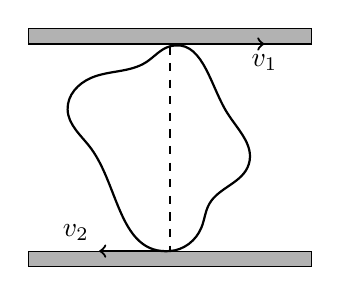
\begin{tikzpicture}[use Hobby shortcut,closed=true]
    \draw[fill=gray!60] (0.2,0) rectangle ++(3.6,0.2);
    \draw[fill=gray!60] (0.2,2.83) rectangle ++(3.6,0.2);
    \draw[thick] (2,2.8) .. (1.7,2.6) .. (1,2.4) .. (0.7,2) .. (1,1.5)
    .. (2,0.2) .. (2.4,0.5) .. (2.5,0.8) .. (3,1.3) .. (2.7,2)
    .. (2,2.8);
    \draw[dashed] (2,2.8) -- (2,0.2);
    \draw[thick,->] (2,2.83) -- ++(1.2,0) node[below] {$v_1$}; 
    \draw[thick,->] (2,0.2) -- ++(-0.9,0) node[above left] {$v_2$}; 
  \end{tikzpicture}
}

\end{document}


%%% Local Variables: 
%%% mode: latex
%%% TeX-engine:xetex
%%% TeX-PDF-mode: t
%%% End:
